%%%%%%%%%%%%%%%%%%%%%%%%%%%%%%%%%%%%%%%%%
% Short Sectioned Assignment
% LaTeX Template
% Version 1.0 (5/5/12)
%
% This template has been downloaded from:
% http://www.LaTeXTemplates.com
%
% Original author:
% Frits Wenneker (http://www.howtotex.com)
%
% License:
% CC BY-NC-SA 3.0 (http://creativecommons.org/licenses/by-nc-sa/3.0/)
%
%%%%%%%%%%%%%%%%%%%%%%%%%%%%%%%%%%%%%%%%%

%----------------------------------------------------------------------------------------
%	PACKAGES AND OTHER DOCUMENT CONFIGURATIONS
%----------------------------------------------------------------------------------------

\documentclass[paper=a4, fontsize=11pt]{scrartcl} % A4 paper and 11pt font size

\usepackage[T1]{fontenc} % Use 8-bit encoding that has 256 glyphs
\usepackage{fourier} % Use the Adobe Utopia font for the document - comment this line to return to the LaTeX default
\usepackage[spanish]{babel} % English language/hyphenation
\usepackage[utf8x]{inputenc}
\usepackage{lipsum} % Used for inserting dummy 'Lorem ipsum' text into the template
\usepackage{graphicx}
\graphicspath{ {images/} }
\usepackage{sectsty} % Allows customizing section commands
\allsectionsfont{\centering \normalfont\scshape} % Make all sections centered, the default font and small caps

\usepackage{fancyhdr} % Custom headers and footers
\pagestyle{fancyplain} % Makes all pages in the document conform to the custom headers and footers
\fancyhead{} % No page header - if you want one, create it in the same way as the footers below
\fancyfoot[L]{} % Empty left footer
\fancyfoot[C]{} % Empty center footer
\fancyfoot[R]{\thepage} % Page numbering for right footer
\renewcommand{\headrulewidth}{0pt} % Remove header underlines
\renewcommand{\footrulewidth}{0pt} % Remove footer underlines
\setlength{\headheight}{13.6pt} % Customize the height of the header


%\setlength\parindent{0pt} % Removes all indentation from paragraphs - comment this line for an assignment with lots of text

%----------------------------------------------------------------------------------------
%	TITLE SECTION
%----------------------------------------------------------------------------------------

\newcommand{\horrule}[1]{\rule{\linewidth}{#1}} % Create horizontal rule command with 1 argument of height

\title{	
\normalfont \normalsize 
\textsc{Universidad de Castilla La Mancha} \\ [25pt] % Your university, school and/or department name(s)
\horrule{0.5pt} \\[0.4cm] % Thin top horizontal rule
\huge Artículo 3. Using OLAP and multidimensional data for decision making \\ % The assignment title
\horrule{2pt} \\[0.5cm] % Thick bottom horizontal rule
}

\author{José María García García} % Your name

\date{\normalsize\today} % Today's date or a custom date

\begin{document}

\maketitle % Print the title

%----------------------------------------------------------------------------------------
%	PROBLEM 1
%----------------------------------------------------------------------------------------

\section{Preguntas}

Leer el artículo y obtener de él información acerca de los siguientes puntos.

\begin{itemize}
\item \textbf{ ¿Qué dos sistemas puede utilizar un gestor para obtener un mejor conocimiento de su empresa?}
\end{itemize}
Procesamiento analítico en línea y Bases de Datos de Múltiples Dimensiones. Estos sistemas nos presentan información resumida que han extraído de las bases de la empresa. Cogen datos sobre el rendimiento de la empresa, los trocean y organizan en estructuras de varias dimensiones y los presentan de manera que permite a los gestores descubrir problemas más rápidamente. 

\begin{itemize}
\item \textbf{¿Qué diferencia hay entre los sistemas OLTP y OLAP?}
\end{itemize}
Los sistemas OLTP son sistemas de procesamiento de transacciones en línea, por lo que están centrados en las operaciones del día a día de la empresa, y no tanto en el análisis de los datos que generan esas transacciones. No obstante, estos sistemas suelen incorporar mecanismos para generar informes según las actividades de la empresa, pero estos no sirven para tener una visión general ni para apreciar rápidamente puntos fuertes y puntos débiles. 

\begin{itemize}
\item \textbf{A la hora de obtener información sobre el funcionamiento general de la empresa, ¿qué características tiene el tipo de sistema preferido 	 por los gestores?}
\end{itemize}
A diferencia del sistema comentado anteriormente, un sistema que usa OLAP y MDDB es intuitivo, fácil de usar y está orientado a la busqueda de información de tal forma que permita, mediante un vistazo rápido, saber que está pasando en la empresa y formarse una idea general sobre la misma.
%%%%%%%%%%%%%%%% OJO A JUGAR PARA LAS COMILLAS DOBLES
\begin{itemize}
\item \textbf{¿Cómo se representa la información cuando utilizamos una base de datos multidimensional?. Indica un ejemplo}
\end{itemize}
La información se representa mediante arrays (vectores, listas) de varias dimensiones. A la estructura que toman los datos en la base se la llama \textbf{hipercubo}, aunque esta puede no tener forma de cubo, esto es, si el array en cuestión tiene una dimensión 4, no podemos representar esa estructura como un tetraedro, ya que para ello el array debería ser de dimensión 3. Estas estructuras son preferidas a otras porque permiten ``jugar'' con la información para observarla desde muchos puntos de vista diferentes, centrar el análisis en un único aspecto de los datos, etc. El uso más simple de estas bases es el que podemos observar en el ejemplo.
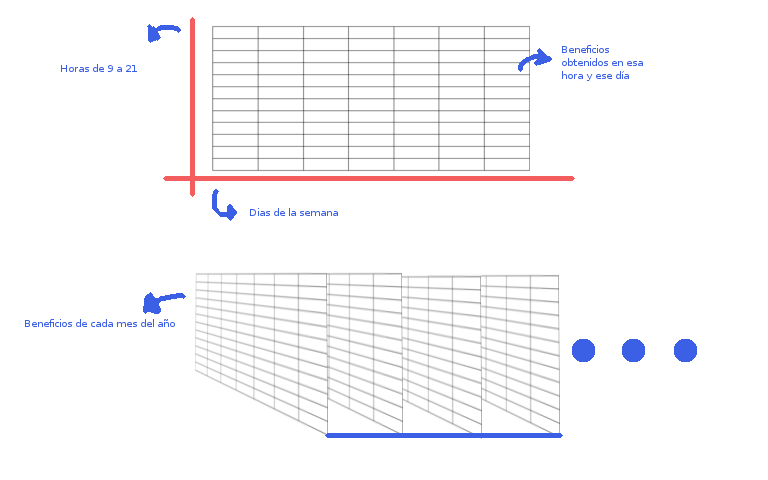
\includegraphics[scale=0.75]{ejemplo}
\newline
En este caso, el dato a estudiar ha sido el beneficio que obtiene la empresa y las variables según las cuales lo hemos estudiado han sido la hora del día, el día de la semana y el mes del año. Esta representación permite ver como varían los datos según cada una de las variables, localizar los puntos donde se detecten perdidas y arreglarlos, etc. Cabe también destacar que cada valor de beneficio está identificado de forma unívoca por sus coordenadas en el cubo (mes, día, hora).


\begin{itemize}
\item \textbf{¿Por qué las base de datos relacionales son adecuadas para almacenar información transaccional y no analítica?}
\end{itemize}
Porque estas bases permitían guardar información de las transacciones de forma rápida y sencilla, información que luego se podía estudiar con los informes autogenerados o a través de órdenes SQL. No obstante, dada la fragmentación y volumen que presentan los datos usados en analítica, manejar estas bases de datos dejaba de ser una trivialidad, por lo que para analítica se prefieren las MDDB.

\begin{itemize}
\item \textbf{ ¿Qué tipo de información suele almacenarse en las base de datos multidimensionales?}
\end{itemize}
Los datos comúnmente almacenados en estas bases de datos suelen ser numéricos y muestran el rendimiento que ha tenido la empresa u organización a lo largo de su historia. Estos datos provienen de otras bases de la empresa, que se vuelcan en la base multidimensional y esta limpia, resume y procesa la información para el uso de los gestores.

\begin{itemize}
\item \textbf{ ¿Qué tipo de interactividad es permitida sobre los datos de una base de datos multidimensional?¿Qué tipo de aplicaciones permiten esta interactividad?}
\end{itemize}
Siguiendo la metáfora del cubo respecto a la representación de la información, el cubo puede hacerse rodajas, para observar los valores de los datos respecto a un valor concreto de una de las coordenadas de los mismos. Estas rodajas pueden trocearse además para observar la información enmarcada en un rango de valores. Podemos observar cuadrados concretos del cubo o subconjuntos del mismo. Podemos pasar el cubo por un filtro para quedarnos con los bloques que satisfagan ese filtro. Normalmente esto se hace mediante interfaces gráficas, lo que hace el análisis más ameno que la lectura de un informe. Al conjunto de herramientas que se usan para esa manipulación del cubo se les llama OLAP. 

\begin{itemize}
\item \textbf{¿Qué opciones tenemos a la hora de implantar una MDDB? ¿En qué se centra cada una de ellas?}
\end{itemize}
Existen dos enfoques a la hora de implementar una MDDB:
\begin{enumerate}
\item \underline{Enfoque top-down (de arriba a abajo)}: centrado en la planificación del negocio.
\item \underline{Enfoque bottom-up (de abajo a arriba)}: centrado en bases y sistemas existentes.
\end{enumerate}

\begin{itemize}
\item \textbf{ ¿En qué consiste el ``síndrome de los datos disponibles''?}
\end{itemize}
Es un síndrome en el que se puede caer al usar como enfoque de implementación el bottom-up, que implica que al partir de datos y sistemas que ya existen, se intenta crear una base que lo contenga todo y lo tenga disponible para todos, cuando realmente eso no es necesario.

\begin{itemize}
\item \textbf{ ¿Qué pasos se dan en una implantación top-down?}
\end{itemize}
En este proceso de implementación se empieza desde arriba, es decir, partimos de lo que la empresa quiere y para que lo quiere. Se lleva a cabo una elicitación de requisitos y el desarrollador prepara un prototipo de MDDB que muestra a la empresa haciendo uso de un software OLAP. Este enfoque asegura que la base que se desarrolle se ajustará a las necesidades de la empresa, lo que no siempre es bueno, ya que la base se desarrollará para un fin concreto, además de que se hará sin tener en cuenta los sistemas sobre los que se apoya, lo que puede dar lugar a problemas si estos no se prevén durante el desarrollo. 

\begin{itemize}
\item \textbf{¿Qué pasos se dan en una implantación bottom-up?}
\end{itemize}
	En una implementación partimos de unos datos que ya existen en unas bases de datos de una tecnología completa. El primer paso es analizar dichos datos y tomar medidas para la confección de la base de datos relacional. Esta toma de medidas da lugar a lo que se conoce como diagrama en estrella, que contiene dos tipos de tablas:
	-Tabla de hecho, formada por datos numéricos que existen dentro de la base de datos
	-Tablas de dimensiones, formadas por datos más descriptivos que se pueden asociar a las dimensiones de la base dentro de la empresa.
Este diagrama se usa para traducir la base de datos relacional a una MDDB, ya que permite concretar el tema central del análisis. Esta traducción es también una simplifación y puede incluso automatizarse. 

\begin{itemize}
\item \textbf{¿Qué enfoque alternativo puede plantearse? ¿En qué consiste?}
\end{itemize}


%------------------------------------------------



\section{Lists}

%------------------------------------------------

\subsection{Example of list (3*itemize)}

%------------------------------------------------

\subsection{Example of list (enumerate)}
\begin{enumerate}
\item First item in a list 
\item Second item in a list 
\item Third item in a list
\end{enumerate}

%----------------------------------------------------------------------------------------

\end{document}